This section discusses the effects of independent SARSA learning.
\subsubsection{1 predator vs. 1 prey}
Again, it is interesting to see if independent SARSA works well with the new environment. Te test this, the new environment executed a game of 1 predator vs. 1 prey. The results can be found in figure \ref{graph:sarsa1vs1}.

\begin{center}
	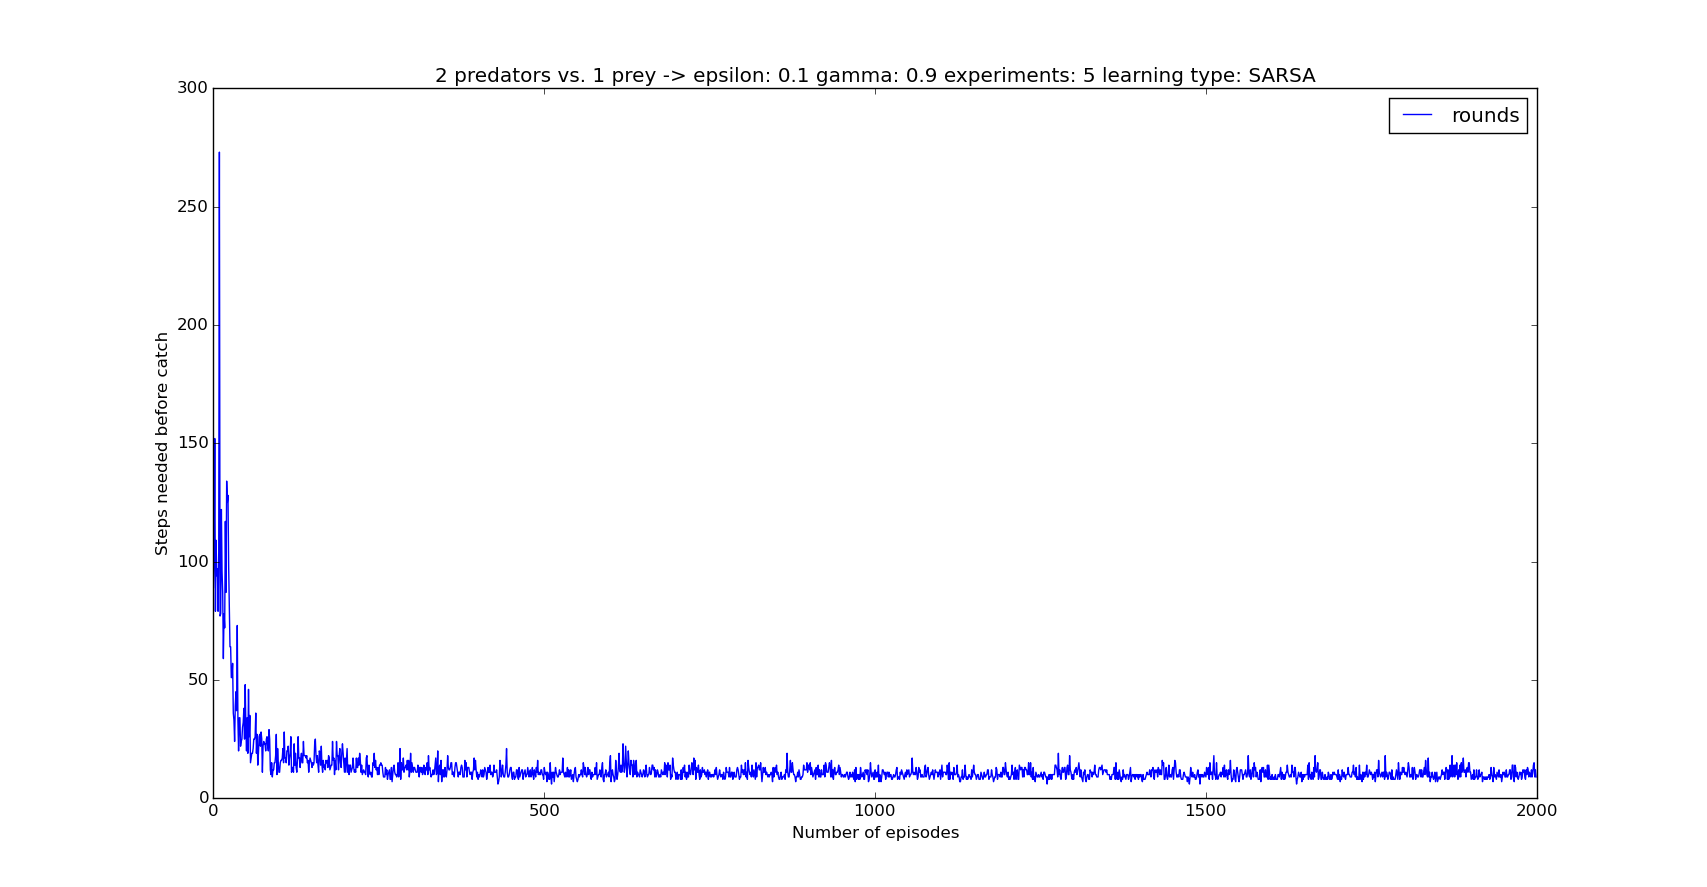
\includegraphics[scale=0.3]{1_predator_1_prey_SARSA}
	\captionof{figure}{Independent SARSA: 1 predator vs. 1 prey}
	\label{graph:sarsa1vs1}
\end{center}

As seen with independent Q-learning, the predator learns how to catch the prey quicker than before. This confirms the theory that the smaller state space leads to quicker convergence of the algorithms. 

Compared to independent Q-learning, SARSA takes much longer to catch the prey in the beginning. Also, after learning the amount of rounds it takes the predators to catch the prey still vary much. However, Q-learning tends to peak in number of rounds to catch the predator after convergence. This does not happen with SARSA, due to the fact that SARSA is more careful than Q-learning. As SARSA is an on-policy learning algorithm, it is more careful than Q-learning. This leads to less extreme exploratory actions, choosing the "safe path" more often than Q-learning.

\subsubsection{2 predators vs. 1 prey}
\begin{center}
	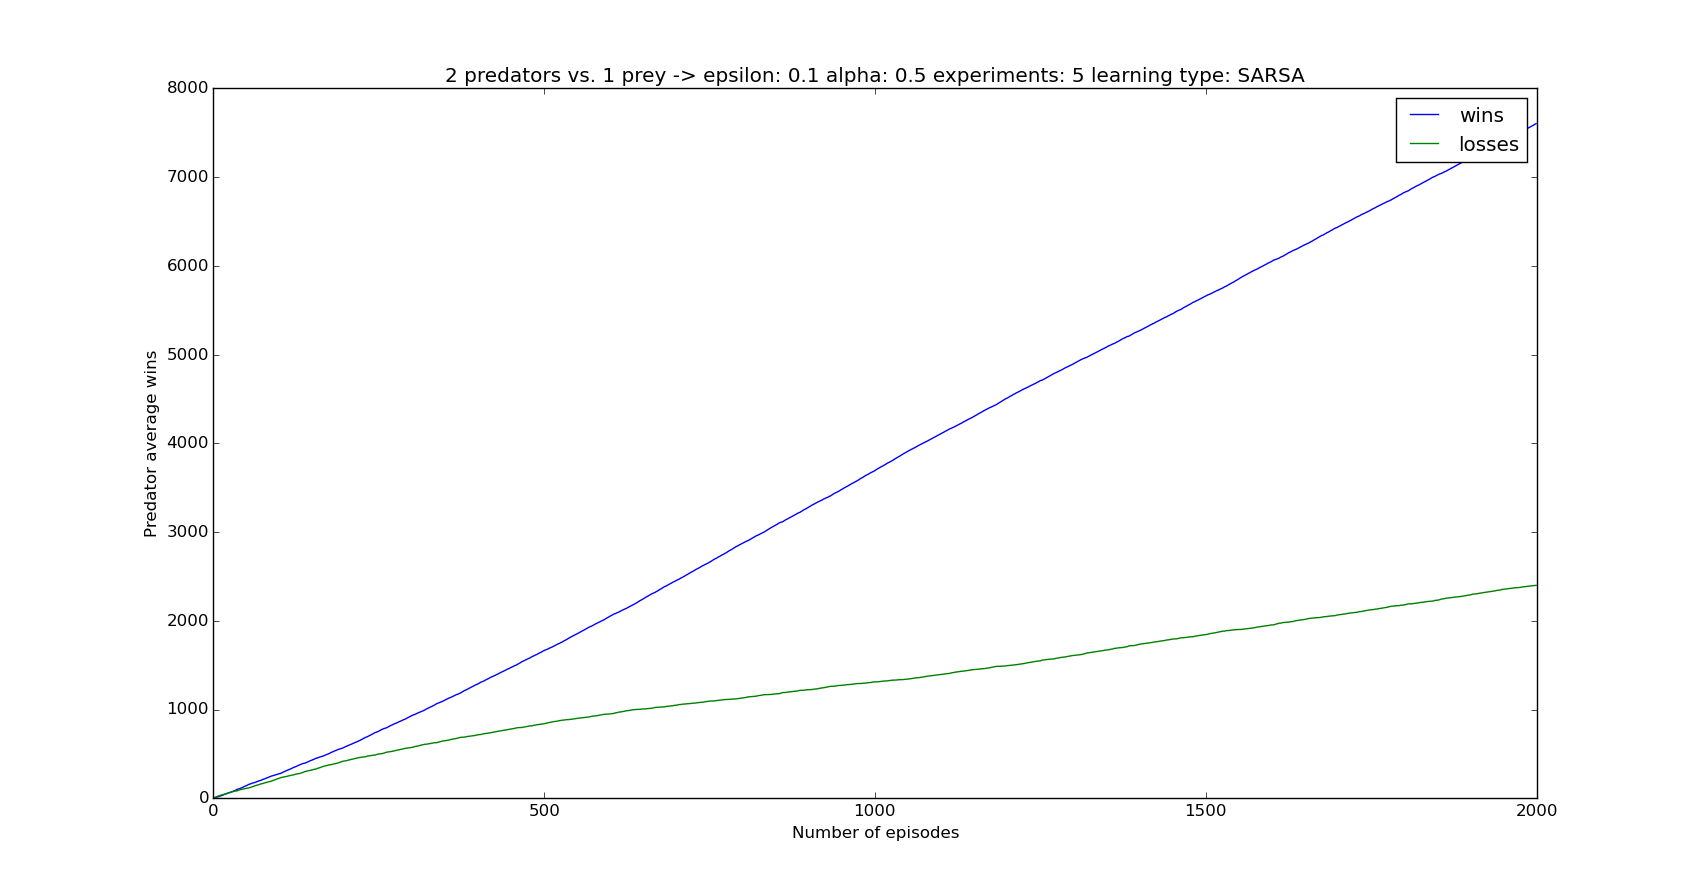
\includegraphics[scale=0.3]{2_predators_SARSA}
	\captionof{figure}{Independent SARSA: 2 predators vs. 1 prey}
	\label{graph:sarsa2vs1}
\end{center}

The graph shown in figure \ref{graph:sarsa2vs1} is very similar to the corresponding graph for Q-learning. This is possible, as both are temporal difference learning methods and are based on the same principles. The main difference between these two is that SARSA is an on-policy learning method and Q-learning is an off-policy learning method. It is therefore expected for these two methods to behave similarly.

\begin{table}[H]
\begin{center}
\begin{tabular}{| l | l | l | l | l |}
\hline
 & \parbox{2cm}{\textbf{Avg wins \\ (first 100)}} & \parbox{2cm}{\textbf{Avg losses \\ (first 100)}} & \parbox{2cm}{\textbf{Avg wins \\ (last 100)}} & \parbox{2cm}{\textbf{Avg losses \\ (last 100)}} \\
\hline
\textbf{Predators} & 55 & 44 & 78 & 21 \\
\hline
\end{tabular}
\caption{Average number of wins and losses by the predators}
\end{center}
\end{table}

Compared to independent Q-learning, independent SARSA performs slightly better. This can be attributed to the fact that SARSA is more careful than Q-learning. This behaviour leads to more wins for the predators, on average, compared to Q-learning.

\subsubsection{3 predators vs. 1 prey}
It is interesting to see what happens when three predators take on one prey. As seen with independent Q-learning, this does not work well. As SARSA is a more careful algorithm, the predators may learn to cooperate better than with Q-learning.

\begin{center}
	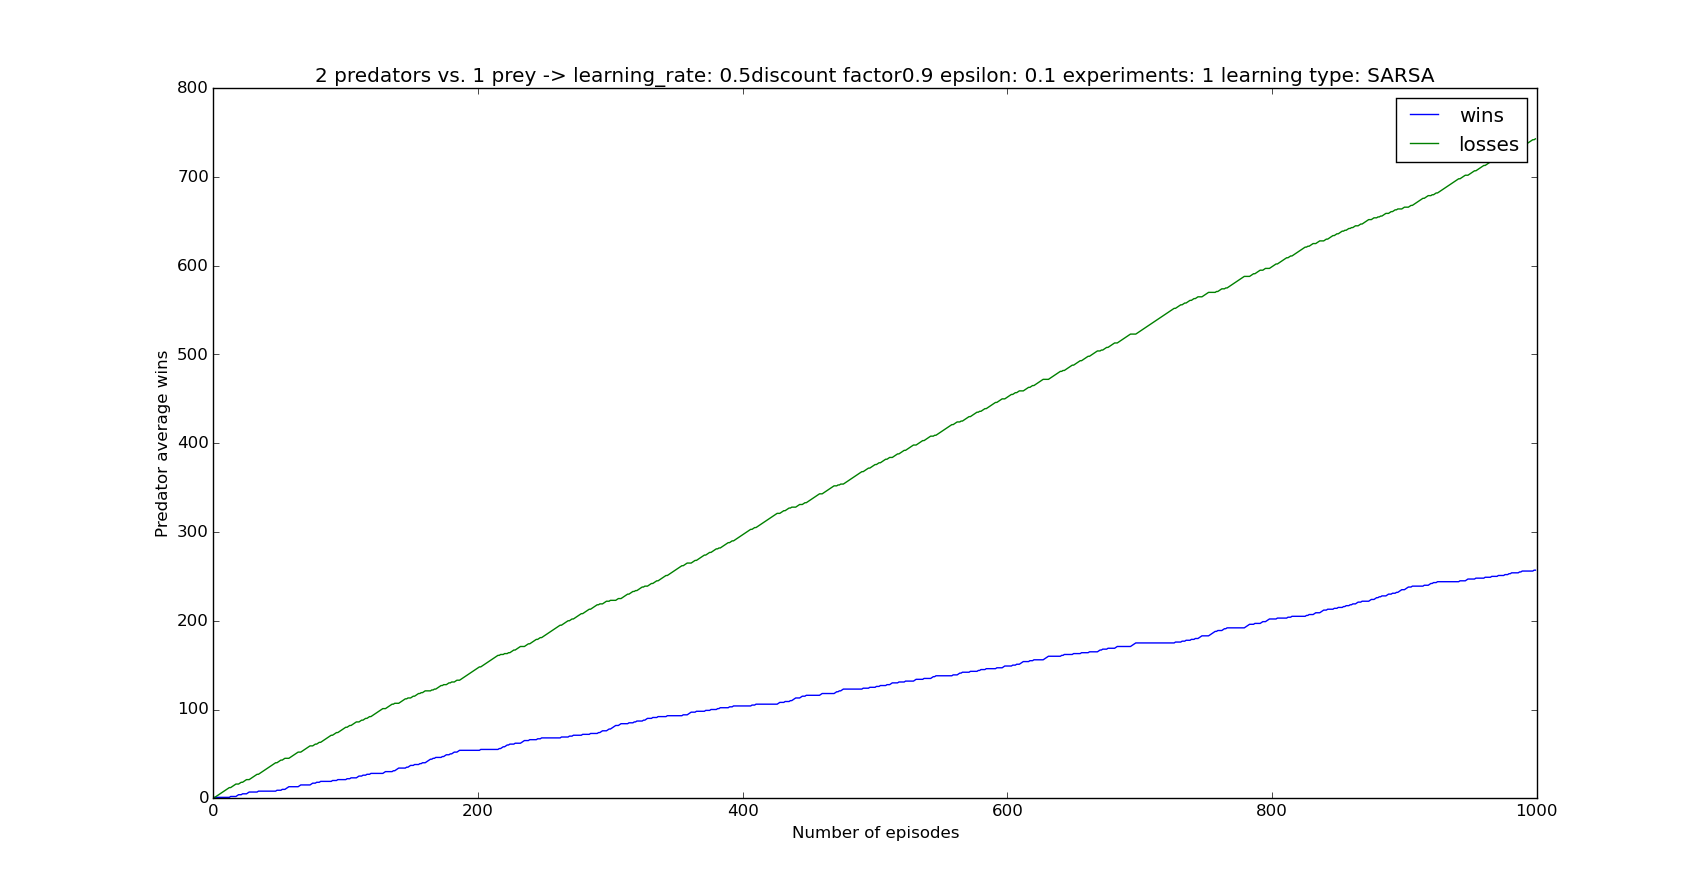
\includegraphics[scale=0.3]{3_predators_SARSA}
	\captionof{figure}{Independent SARSA: 3 predators vs. 1 prey}
	\label{graph:sarsa3vs1}
\end{center}


The graph in figure \ref{graph:sarsa3vs1} shows that the prey manages to escape most of the times.\labelerrorfootnote \: This hardly differs from independent Q-learning.

\begin{table}[H]
\begin{center}
\begin{tabular}{| l | l | l | l | l |}
\hline
 & \parbox{2cm}{\textbf{Avg wins \\ (first 100)}} & \parbox{2cm}{\textbf{Avg losses \\ (first 100)}} & \parbox{2cm}{\textbf{Avg wins \\ (last 100)}} & \parbox{2cm}{\textbf{Avg losses \\ (last 100)}} \\
\hline
\textbf{Predators} & 21 & 79 & 22 & 77 \\
\hline
\end{tabular}
\caption{Average number of wins and losses by the predators with varying learning rates}
\end{center}
\end{table}

This shows that SARSA learns very slowly, in this case. Combined with the fact that there are many predators on a small grid, these can bump into one another. Any learning will be much delayed. It is important to note that this is the only test which was run once, with 1000 episodes.

\subsubsection{4 predators vs. 1 prey}
Just like performing Q-learning with 4 predators and 1 prey, this case is again intractable. More information about the problem might be found in section \ref{sec:intractable}.

\subsubsection{Parameter settings}
Again, parameter settings were explored for this algorithm. This was tested with two predators and one prey.

\subsubsection{Learning rate}
First, the effect of the learning rate is researched. As the learning rate determines to what extent the newly acquired information will override the old information, it is interesting to see what happens. 

\begin{center}
	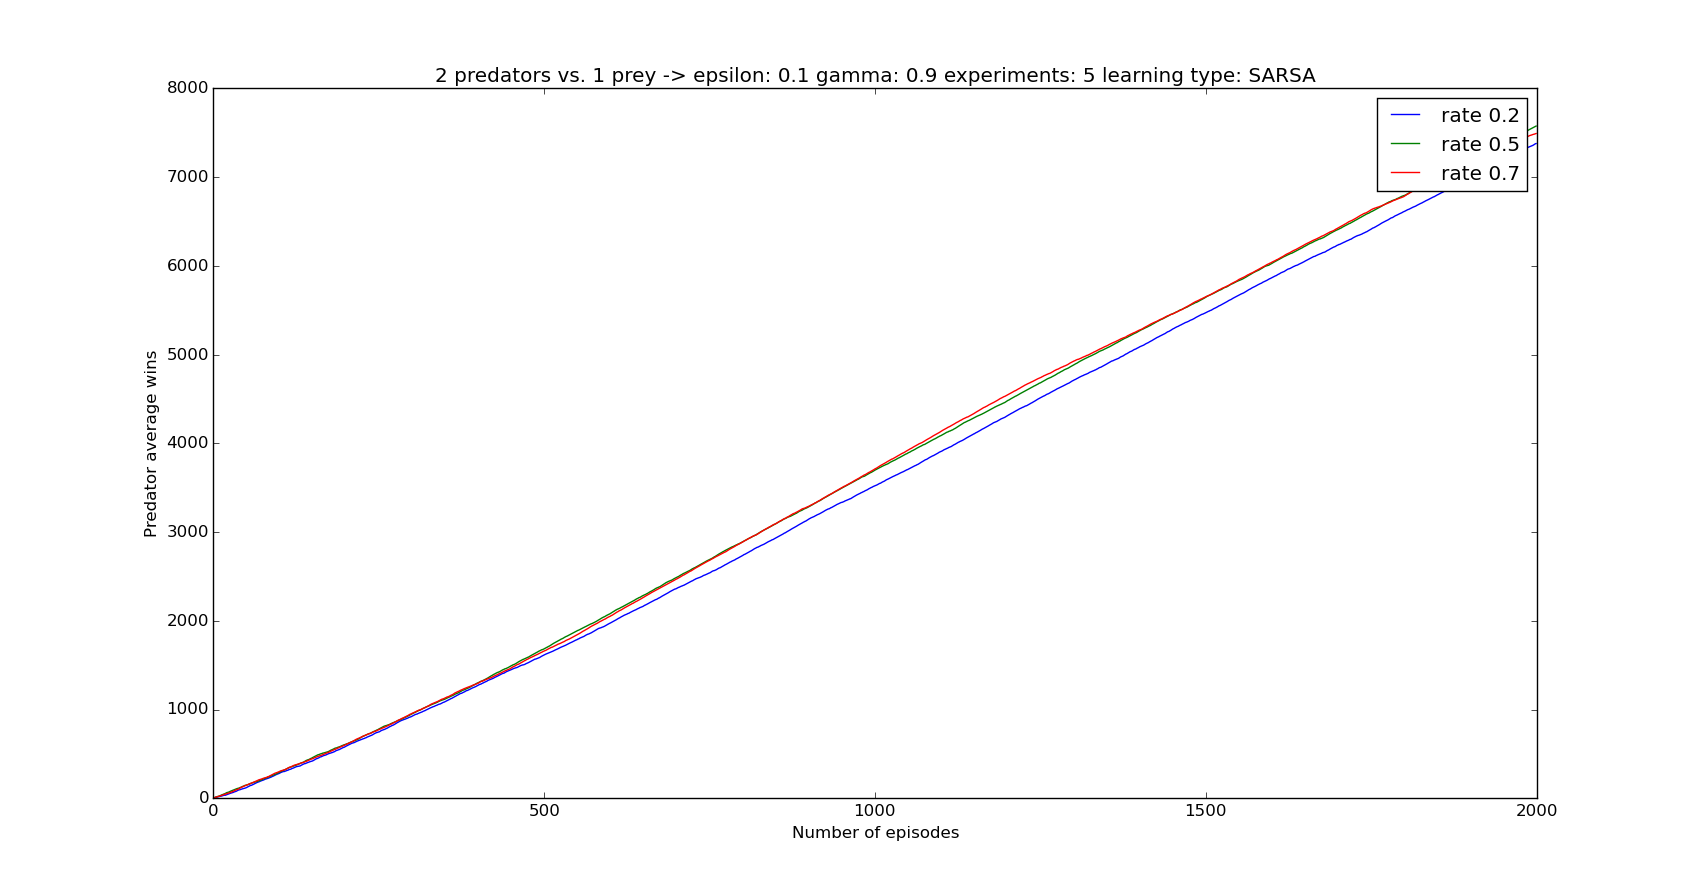
\includegraphics[scale=0.3]{2_predators_learning_rate_SARSA}
	\captionof{figure}{Independent SARSA: 2 predators vs. 1 prey, learning rate}
	\label{graph:sarsalearningrates}
\end{center}

From the graph in figure \ref{graph:sarsalearningrates} it is difficult to see if a high or average learning rate affect the implementation in the best possible way. In the end, however it appears as though a learning rate of 0.5 yields best results.

\begin{table}[H]
\begin{center}
\begin{tabular}{| l | l | l | l | l |}
\hline
\parbox{2cm}{\textbf{Learning rate}} & \parbox{2cm}{\textbf{Avg wins \\ (first 100)}} & \parbox{2cm}{\textbf{Avg losses \\ (first 100)}} & \parbox{2cm}{\textbf{Avg wins \\ (last 100)}} & \parbox{2cm}{\textbf{Avg losses \\ (last 100)}} \\
\hline
\textbf{0.2} & 56 & 44 & 75 & 23 \\
\hline
\textbf{0.5} & 58 & 41 & 79 & 19 \\
\hline
\textbf{0.7} & 59 & 40 & 68 & 30 \\
\hline
\end{tabular}
\caption{Average number of wins and losses by the predators with varying learning rates}
\label{table:sarsalearningrates}
\end{center}
\end{table}

Table \ref{table:sarsalearningrates} confirms the theory derived off the graph. A medium learning rate does yield best results. When the predators are learning while hunting the prey, an equal balance of new and old information yields optimal results.

\subsubsection{Discount factor}
The discount factor determines the importance of future rewards. In the previous assignment, a high discount factor yielded best results. This means that the future reward was most important. Only the goal state yielded a reward, making reaching the goal state very important. Currently, there are two terminal states: the win state and the lose state. It is interesting to see what effect the negative rewards have on the importance of the immediate reward.

\begin{center}
	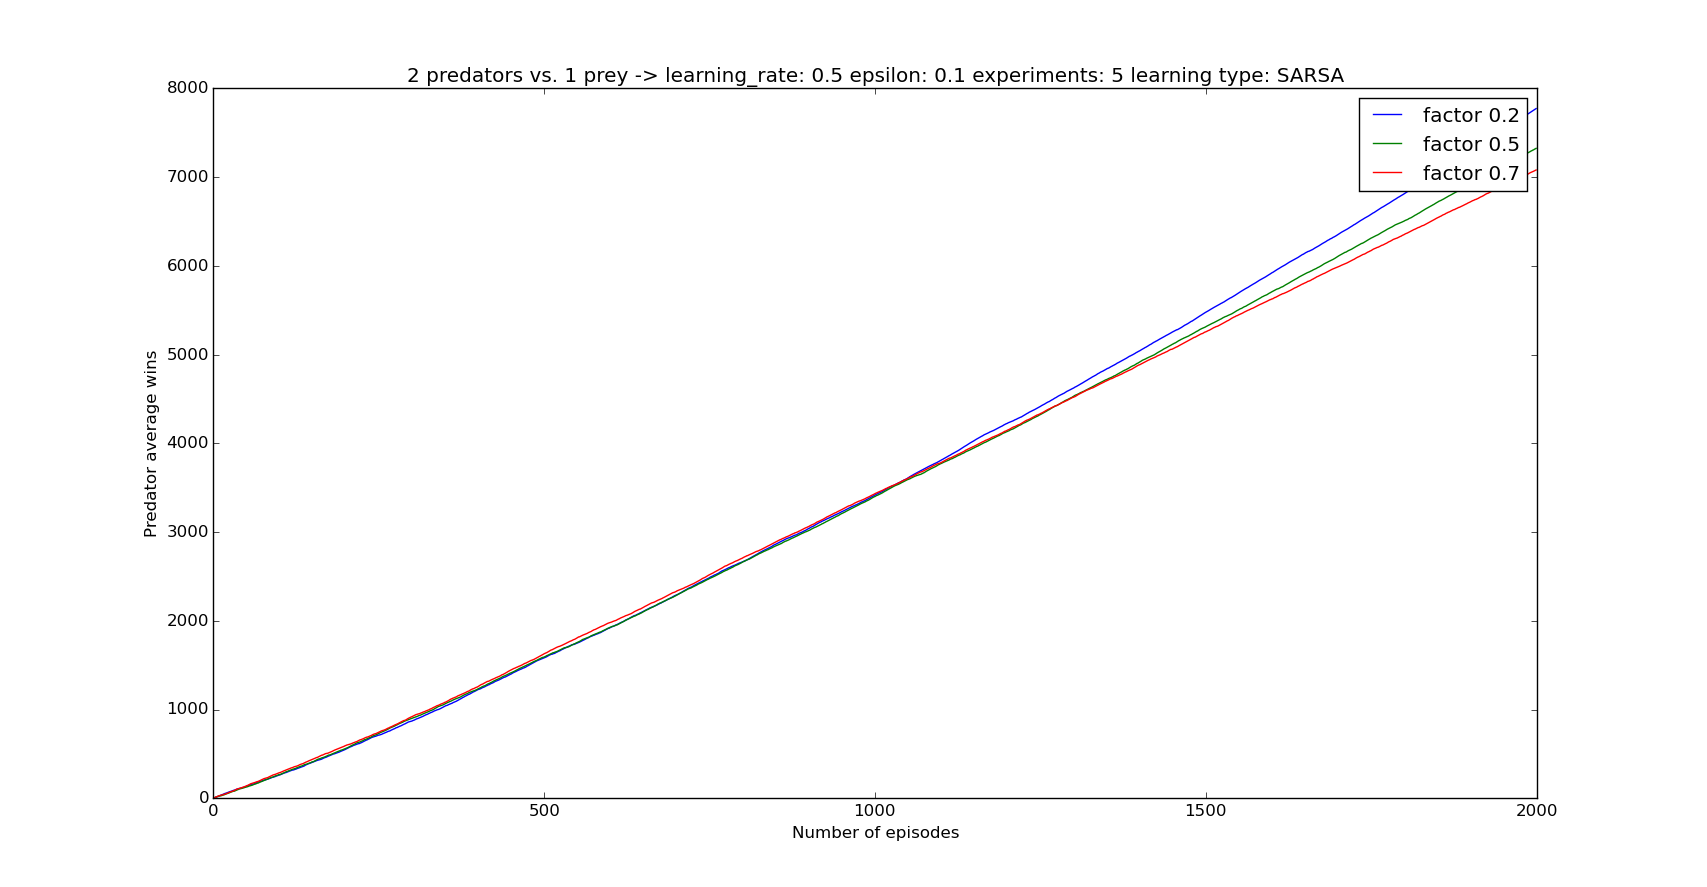
\includegraphics[scale=0.3]{2_predators_discount_factor_SARSA}
	\captionof{figure}{Independent SARSA: 2 predators vs. 1 prey, discount factor}
\end{center}

Again, the immediate reward shows to be important. It has been mentioned several times that SARSA is a careful algorithm, as it collects rewards during learning. Independent Q-learning yields similar results, confirming the theory that introducing a negative reward into the game makes the immediate reward more important.

\begin{table}[H]
\begin{center}
\begin{tabular}{| l | l | l | l | l |}
\hline
\parbox{2cm}{\textbf{Discount factor}} & \parbox{2cm}{\textbf{Avg wins \\ (first 100)}} & \parbox{2cm}{\textbf{Avg losses \\ (first 100)}} & \parbox{2cm}{\textbf{Avg wins \\ (last 100)}} & \parbox{2cm}{\textbf{Avg losses \\ (last 100)}} \\
\hline
\textbf{0.2} & 52 & 47 & 95 & 3 \\
\hline
\textbf{0.5} & 53 & 46 & 80 & 18 \\
\hline
\textbf{0.7} & 57 & 42 & 71 & 27 \\
\hline
\end{tabular}
\caption{Average number of wins and losses by the predators with varying discount factors}
\label{table:sarsadiscountfactor}
\end{center}
\end{table}

The previous conclusions are supported by table \ref{table:sarsadiscountfactor}. However, it is interesting to note that keeping into account the immediate reward yields significantly better results than seen before. Winning games 95\% of the time, on average, is highly successful. This means that even when the predators are exploring new paths, the predators hardly ever bump into one another. These are excellent results for any algorithm, let alone an on-policy algorithm.

\subsubsection{$\epsilon$-greedy action selection}
\begin{center}
	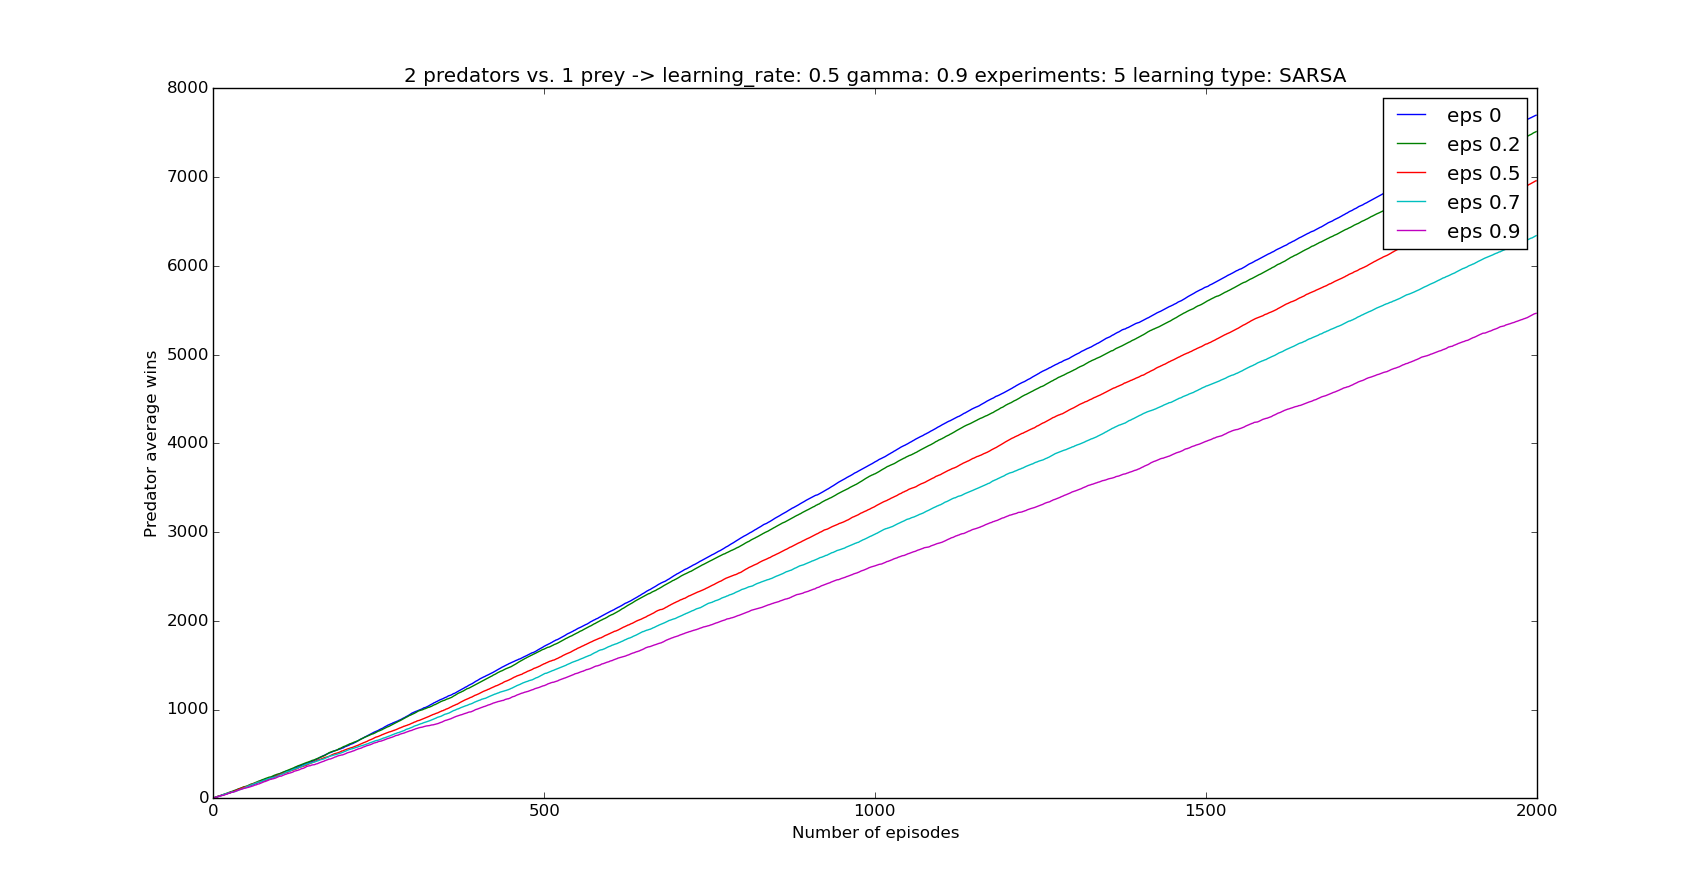
\includegraphics[scale=0.3]{2_predators_epsilon_SARSA}
	\captionof{figure}{Independent SARSA: 2 predators vs. 1 prey, $\epsilon$-greedy action selection}
	\label{graph:sarsagreedy}
\end{center}

Figure \ref{graph:sarsagreedy} shows that low exploration leads to the best results. Again, this is to be expected as exploration most likely will lead to predators bumping into one another.

\begin{table}[H]
\begin{center}
\begin{tabular}{| l | l | l | l | l |}
\hline
\parbox{2cm}{\textbf{$\epsilon$-rate}} & \parbox{2cm}{\textbf{Avg wins \\ (first 100)}} & \parbox{2cm}{\textbf{Avg losses \\ (first 100)}} & \parbox{2cm}{\textbf{Avg wins \\ (last 100)}} & \parbox{2cm}{\textbf{Avg losses \\ (last 100)}} \\
\hline
\textbf{0} & 54 & 45 & 74 & 24 \\
\hline
\textbf{0.2} & 55 & 45 & 74 & 24 \\
\hline
\textbf{0.5} & 53 & 47 & 73 & 25 \\
\hline
\textbf{0.7} & 51 & 48 & 66 & 32 \\
\hline
\textbf{0.9} & 48 & 51 & 57 & 41 \\
\hline
\end{tabular}
\caption{Average number of wins and losses by the predators with varying $\epsilon$-rates}
\label{table:sarsagreedy}
\end{center}
\end{table}

Table \ref{table:sarsagreedy} confirms almost what the graph shows. Where the graph shows better results for an absolutely greedy action selection, the table shows that the results over the last 100 runs are exactly the same.  This will lead to trying to catch the prey in the beginning, but exploring other paths to the prey while avoiding other predators is also important. This can help the predators significantly in the future. However, exploration is needed. Therefore, lowering the learning rate over time will help the predators best. This confirms the theory that the learning rate must be lowered in order to yield best results.